% TLG-mapped BNN tile microarchitecture (Fig. 2).
% Build: pdflatex fig2_tile_microarch.src.tex && mv fig2_tile_microarch.src.pdf fig2_tile_microarch.pdf
\documentclass[border=2pt]{standalone}
\usepackage{mathptmx}
\usepackage{tikz}
\usetikzlibrary{arrows.meta,positioning,calc,fit,backgrounds,decorations.pathreplacing}

\definecolor{navy}{HTML}{1F3A5F}
\definecolor{tlgred}{HTML}{A83232}
\definecolor{redfill}{HTML}{F4DADA}

\begin{document}
% Native width tuned to ~293 pt to match fig1, so when both figures
% are placed at \columnwidth in main.tex, on-paper font sizes match.
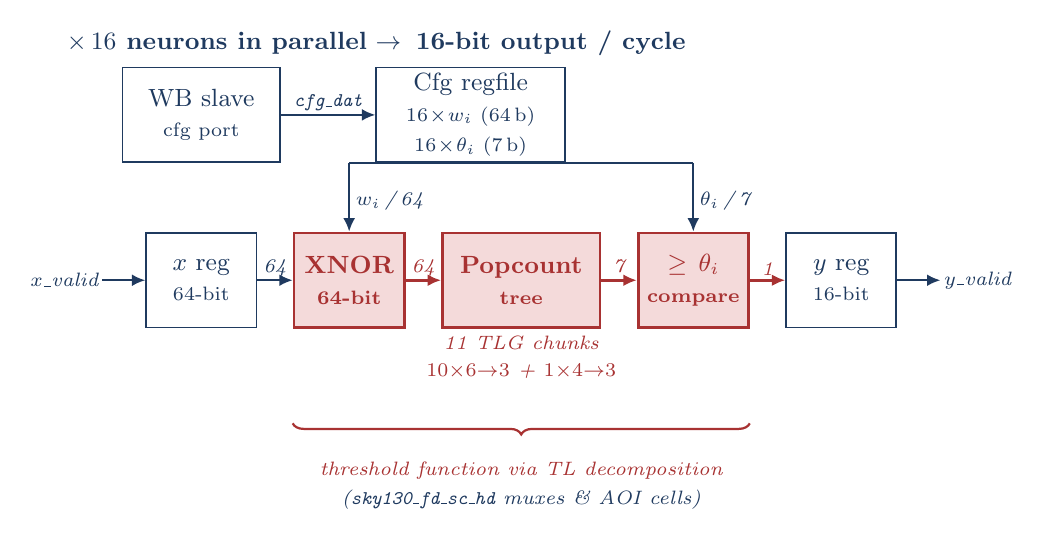
\begin{tikzpicture}[
    font=\rmfamily,
    >={Latex[length=1.7mm,width=1.5mm]},
    line width=0.6pt,
    primary/.style  = {draw=navy, fill=navy, text=white, line width=0.6pt,
                       minimum height=10mm, minimum width=15mm, align=center,
                       inner sep=2pt, font=\rmfamily\small},
    secondary/.style= {draw=navy, fill=white, text=navy, line width=0.6pt,
                       minimum height=10mm, minimum width=14mm, align=center,
                       inner sep=2pt, font=\rmfamily\small},
    tlg/.style      = {draw=tlgred, fill=redfill, text=tlgred, line width=1.0pt,
                       minimum height=10mm, minimum width=14mm, align=center,
                       inner sep=2pt, font=\rmfamily\small\bfseries},
    sig/.style      = {draw=navy, line width=0.8pt, ->},
    redsig/.style   = {draw=tlgred, line width=1.2pt, ->},
    wlbl/.style     = {font=\rmfamily\scriptsize\itshape, text=navy, inner sep=1pt},
    note/.style     = {font=\rmfamily\scriptsize\itshape, text=navy,
                       align=center, inner sep=1pt},
  ]

  % ===================================================================
  % Top row: WB slave + Cfg regfile (well above datapath, with
  % generous gap so the cfg_dat label has breathing room)
  % ===================================================================
  \node[secondary, minimum width=20mm, minimum height=12mm] (wb)
    at (-3.7,2.10) {WB slave\\\scriptsize cfg port};
  \node[secondary, minimum width=24mm, minimum height=12mm,
        anchor=west] (cfg) at ($(wb.east)+(1.20,0)$)
    {Cfg regfile\\\scriptsize $16\!\times\! w_i$ (64\,b)\\\scriptsize $16\!\times\! \theta_i$ (7\,b)};
  \draw[sig] (wb.east) -- (cfg.west)
    node[wlbl, midway, above] {\texttt{cfg\_dat}};

  % ===================================================================
  % Datapath (single horizontal row at y = 0)
  % Layout: x reg → XNOR → Popcount → ≥θ → y reg
  % ===================================================================
  \node[secondary, minimum width=14mm, minimum height=12mm] (xreg)
    at (-3.7,0) {$x$ reg\\\scriptsize 64-bit};

  \node[tlg, minimum width=14mm, minimum height=12mm, anchor=west]
    (xnor) at ($(xreg.east)+(0.45,0)$) {XNOR\\\scriptsize 64-bit};

  \node[tlg, minimum width=20mm, minimum height=12mm, anchor=west]
    (pop) at ($(xnor.east)+(0.45,0)$)
    {Popcount\\\scriptsize tree};

  \node[tlg, minimum width=14mm, minimum height=12mm, anchor=west]
    (cmp) at ($(pop.east)+(0.45,0)$)
    {$\geq\,\theta_i$\\\scriptsize compare};

  \node[secondary, minimum width=14mm, minimum height=12mm, anchor=west]
    (yreg) at ($(cmp.east)+(0.45,0)$) {$y$ reg\\\scriptsize 16-bit};

  % Datapath arrows with explicit bit-widths
  \draw[sig]    (xreg.east) -- (xnor.west) node[wlbl, midway, above] {64};
  \draw[redsig] (xnor.east) -- (pop.west)
    node[wlbl, midway, above, text=tlgred] {64};
  \draw[redsig] (pop.east)  -- (cmp.west)
    node[wlbl, midway, above, text=tlgred] {7};
  \draw[redsig] (cmp.east)  -- (yreg.west)
    node[wlbl, midway, above, text=tlgred] {1};

  % Sub-label under Popcount: chunk decomposition detail
  \node[note, text=tlgred, anchor=north]
    at ($(pop.south)+(0,-0.05)$)
    {\scriptsize 11 TLG chunks};
  \node[note, text=tlgred, anchor=north]
    at ($(pop.south)+(0,-0.40)$)
    {\scriptsize $10{\times}6{\to}3$ + $1{\times}4{\to}3$};

  % ----- Cfg regfile drives w_i / theta_i down -----
  \draw[draw=navy, line width=0.6pt]
    (cfg.south -| xnor.north) -- (cfg.south -| cmp.north);
  \draw[sig] (cfg.south -| xnor.north) -- (xnor.north)
    node[wlbl, pos=0.55, right=1pt] {$w_i$\,/\,64};
  \draw[sig] (cfg.south -| cmp.north) -- (cmp.north)
    node[wlbl, pos=0.55, right=1pt] {$\theta_i$\,/\,7};

  % ----- x_valid in / y_valid out -----
  \draw[sig] ($(xreg.west)+(-0.55,0)$) -- (xreg.west);
  \node[wlbl, anchor=east] at ($(xreg.west)+(-0.55,0)$) {$x\_\textrm{valid}$};
  \draw[sig] (yreg.east) -- ++(0.55,0);
  \node[wlbl, anchor=west] at ($(yreg.east)+(0.55,0)$) {$y\_\textrm{valid}$};

  % ===================================================================
  % TL-decomposition bracket beneath the red blocks
  % ===================================================================
  \draw[decorate, decoration={brace, amplitude=4pt, mirror},
        draw=tlgred, line width=0.8pt]
    ($(xnor.south west)+(0,-1.20)$) -- ($(cmp.south east)+(0,-1.20)$);
  \node[note, text=tlgred, anchor=north]
    at ($(pop.south)+(0,-1.65)$)
    {threshold function via TL decomposition};
  \node[note, anchor=north]
    at ($(pop.south)+(0,-2.00)$)
    {(\texttt{sky130\_fd\_sc\_hd} muxes \& AOI cells)};

  % ===================================================================
  % "× 16 neurons" annotation at top of figure
  % ===================================================================
  \node[note, text=navy, anchor=south, font=\rmfamily\small, align=center]
    at ($(cfg.north)+(-1.2,0.10)$)
    {\textbf{$\times\,16$ neurons in parallel}
     \textbf{$\to$\, 16-bit output / cycle}};

\end{tikzpicture}
\end{document}
